\documentclass[twoside,twocolumn]{article}

\usepackage{blindtext} 
\usepackage{graphicx}
\usepackage[sc]{mathpazo} 
\usepackage[T1]{fontenc} 
\linespread{1.05} 
\usepackage{microtype} 


\usepackage[english]{babel} 


\usepackage[hmarginratio=1:1,top=32mm,columnsep=20pt]{geometry} 
\usepackage[hang, small,labelfont=bf,up,textfont=it,up]{caption} 
\usepackage{booktabs} 


\usepackage{lettrine} 


\usepackage{enumitem} 
\setlist[itemize]{noitemsep} 


\usepackage{abstract} 
\renewcommand{\abstractnamefont}{\normalfont\bfseries} 
\renewcommand{\abstracttextfont}{\normalfont\small\itshape} 


\usepackage{titlesec} 
\renewcommand\thesection{\Roman{section}} % 
\renewcommand\thesubsection{\roman{subsection}} 
\titleformat{\section}[block]{\large\scshape\centering}{\thesection.}{1em}{} 
\titleformat{\subsection}[block]{\large}{\thesubsection.}{1em}{} 


\usepackage{fancyhdr} 
\pagestyle{fancy} 
\fancyhead{} 
\fancyfoot{} 
\fancyhead[C]{Trabajo de la Unidad I: Proyecto TREVA $\bullet$ Junio 2020 $\bullet$ } 
\fancyfoot[RO,LE]{\thepage} 


\usepackage{titling} 


\usepackage{hyperref} 


%----------------------------------------------------------------------------------------
%	TILULOS
%----------------------------------------------------------------------------------------


\setlength{\droptitle}{-4\baselineskip} 

\pretitle{\begin{center}\Huge\bfseries} 
\posttitle{\end{center}} 
\title{Implementación de Call Center y asistencia para el poder judicial} 
\author{Samuel  - Franklin Carlos, Huichi Contreras, \\
Anthony Robles Flores. }
\date{\today} 
\renewcommand{\maketitlehookd}{
\begin{abstract}
\noindent 
Determino las estrategias que debiera tenerse en cuenta para planificar, estructurar y finalmente escribir un articulo o “paper” de Ciencias Sociales
conforme a la Asociacion Americana de Psicologa (APA) Sexta Edicion. Se pretende que el lector produzca su propio trabajo.
\end{abstract}
\begin{abstract}
\noindent 

Treva es un sistema enfocado en los formularios de satisfacion del cliente en donde el propietario podra generar formularios y enviar cada cierto tiempo a sus empleado o interesados para que puedan llenarlo segun
las opciones que cuenta el formulario, a partir de esos datos podemos al propietario dar estadisticas en la cual puede verificar que opciones escogieron los clientes o empleados, y aparte de ello podemos analizar los datos
para dar recomendaciones o proyecciones estimadas de areas especificas.

\end{abstract}
}

%----------------------------------------------------------------------------------------

\begin{document}

% Print the title
\maketitle

%----------------------------------------------------------------------------------------
%	INTRODUCCION
%----------------------------------------------------------------------------------------

\section{Introduccion}
\lettrine[nindent=0em,lines=3]{L}os centros de llamada operadas o de contacto  hoy en dia por personal es una proveedora de servicios que se encarga de dar soporte y administrar dependiendo los servicios o solicitudes que las empresas proveen. Estos Centros de contactos normalmente son operados en instalaciones que cuentan con equipos como computadoras, telefonos, microfonos,etc. Estos centros suelen estar conectados con algun otro centro o tambien son prestadoras de servicios de estaciones ya establecidas.\\
Actualmente las mas reconocidas e importantes empresas usan centros de contacto para realizar una interaccion con los clientes entre ellos podemos 
contar firmas para pedidos por catalogo, soportes operativos, atencion al cliente, etc.

\section{Planteamiento del problema}
\subsection{Problema}
La problematica general es el como las empresas evaluan el desempeño de sus servicios, y como pueden medir la satisfacción del cliente al igual de saber la efectividad y el buen manejo de sus productos.

\subsection{Justificacion}
Hoy en día los datos toman cada vez mas valor en una organizacion o empresa, de esta manera pueden asegurar una ventaja contra sus competidores y así beneficiarce para obtener una mejor calidad de servicio, mejorar su producto y por consiguiente clientes satisfechos.

\subsection{Alcance}
Para el alcance de este proyecto nesecitaremos de clientes que quieran realizar sus formularios de satisfaccion y ofrecerles todas las herramientas nesecarias para que lo hagan de manera eficaz. Alcanzado la meta podremos generar los dashboards que ayude al cliente a ver los resultados entre otros indicadores.


\section{Objetivos}
\subsection{General}
Determinar el nivel de satisfaccion de los clientes de las empresas afiliadas a treva

\subsection{Especificos}
\begin{itemize}
\item Mejorar el rendimiento de las empresas con reportes estadisticos en las encuestas realizadas sobre el nivel de satisfaccion de los clientes, que se usaran para la toma de desiciones.
\item Comparar los grados de satisfacción de los clientes periodicamente.
\item Definir la relación real entre encuestas y satisfacción del cliente.
\end{itemize}

\section{Referentes teoricos}
La idea nos nacio como grupo luego de ver ejemplos de paginas como bimatico en donde manejaban estadisticas de la realizacion de las estadisticas de cada pregunta y area realizada
a continuacion pondre un ejemplos realizados esta pagina. Apartir de esas estadisticas nos dimos cuenta que pdoriamos realizar un sistema que pueda controlar todo esto desde el punto inicial hasta llegar al punto de los reportes.
\begin{figure}[h!]
	\begin{center}
		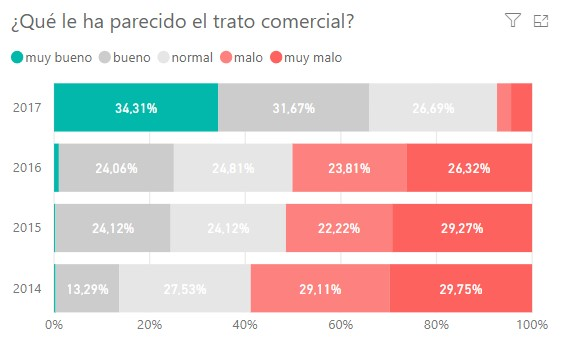
\includegraphics[width=7.5cm]{./Imagenes/esta1} 
		\caption{Estadistica de bimatico}
	\end{center}
\end{figure}
\begin{figure}[h!]
	\begin{center}
		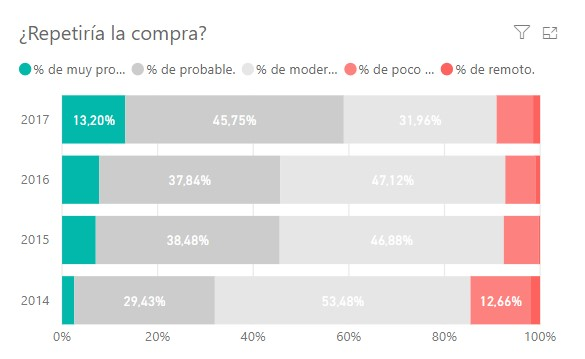
\includegraphics[width=7.5cm]{./Imagenes/esta2} 
		\caption{Estadistica de bimatico}
	\end{center}
\end{figure}
\begin{figure}[h!]
	\begin{center}
		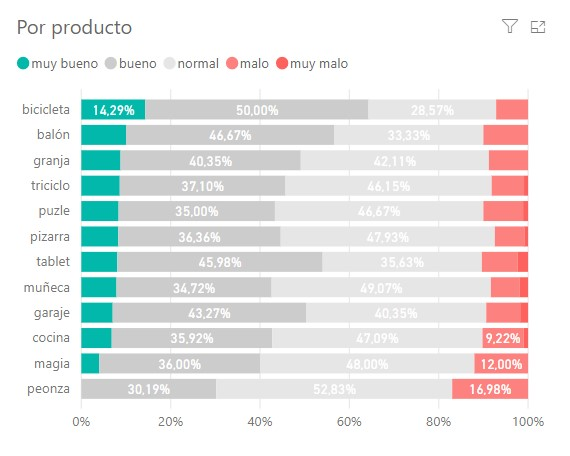
\includegraphics[width=7.5cm]{./Imagenes/esta3} 
		\caption{Estadistica de bimatico}
	\end{center}
\end{figure}

\section{Desarrollo de la propuesta}
Para solucionar nuestra problematica hemos desarrollado una propuesta la cual consiste en la creacion de encuestas de satifaccion mediante formularios web para los clientes usuarios de una empresa u organizacion. Para esto se creara una plataforma movil y web en la cual se podra crear, modificar y eliminar encuestas de satisfaccion personalizadas para cada empresa. El sistema evaluara esas encuestas y realizara un estudio de Inteligencia de Negocios para brindar datos de valor a la empresa u organizacion involucrada, de esta forma se busca ayudar en la toma de desiciones y mejorar la calidad de servicio.

\subsection{Tecnologia de informacion}
En esta sección definiremos las herramientas tecnologicas utilizadas para la realizacion del proyecto.
\begin{itemize}
\item Gestor de Archivos:
\subitem Github.
\item Hosting:
\subitem Hostgator.
\item Base de Datos:
\subitem MySQL.
\item Lenguajes de programación:
\subitem JavaScript.
\subitem PHP.
\item Librerias:
\subitem VueJs.
\subitem Bootstrap.
\subitem Axios.
\subitem ReactNative.
\subitem SweerAlert2.
\item Reportes:
\subitem Highchart.
\item Seguridad:
\subitem Google reCaptcha v3.
\end{itemize}

\subsection{Metodologia, tecnicas usadas}
La metodologia que usamos para la realizacion es una combinacion de Scrum y Kanban, por el lado de scrum realizamos historias de usuario y el product backlog, como tambien la division de tareas y su estimacion de importancia y tiempo. En medio del sprint usamos kanban para realizar una tabla en la cual se pondria todas las tareas que se realizarian en cada Sprint, haciendo reunionnes en cada oportunidad que tengamos para ir viendo el avanze del proyecto y su continuacion y mejora de ello. Estas tecnicas fueron escogidas por el grupo debido al tiempo que manejabamos y disponiamos en las horas de clase.

\section{Cronograma}
\begin{figure}[htb]
	\begin{center}
		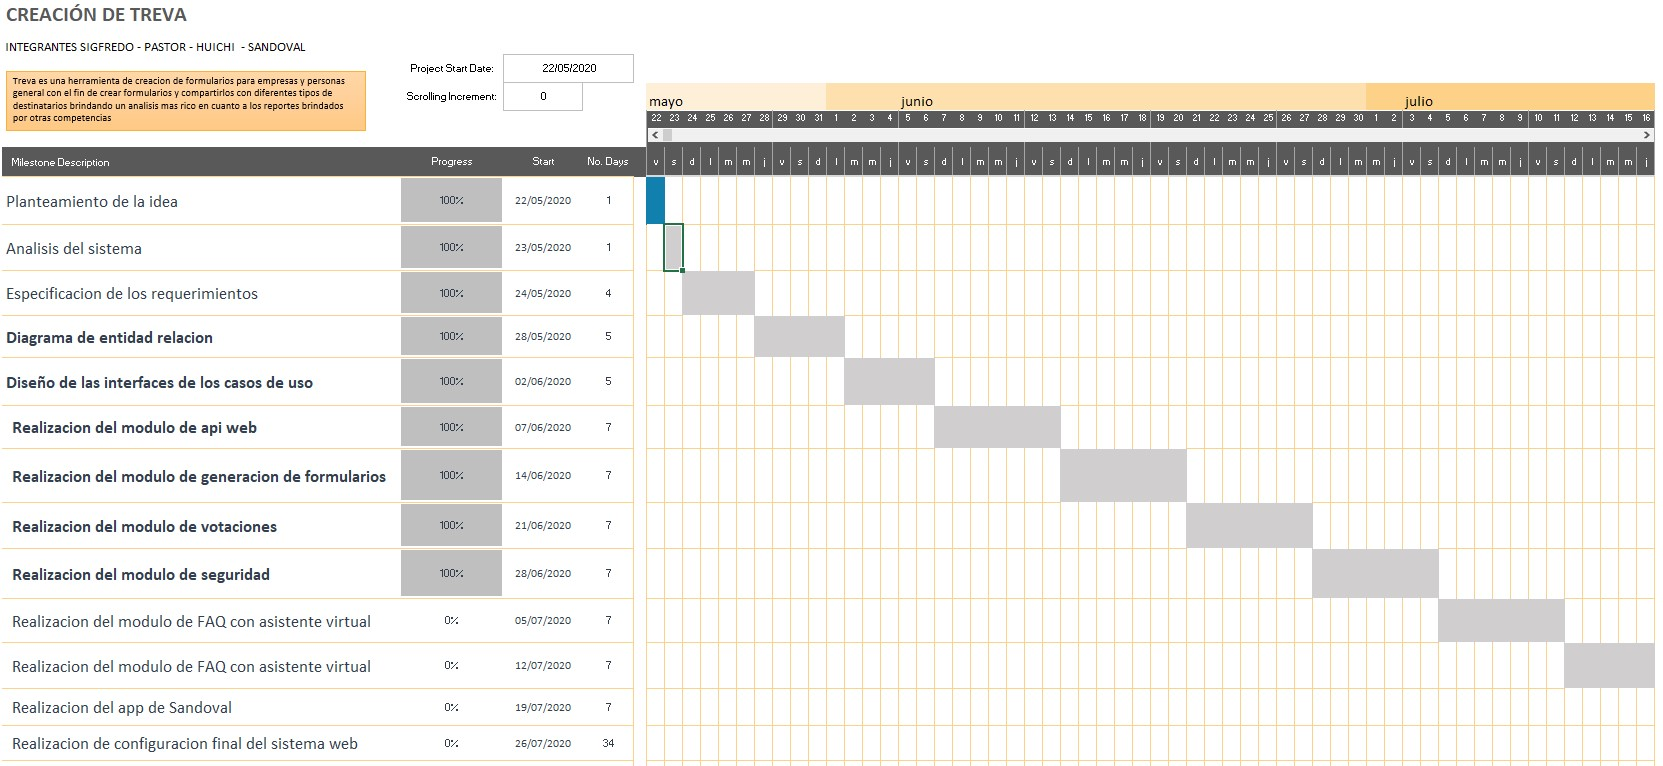
\includegraphics[width=7.5cm]{./Imagenes/Cronograma} 
		\caption{Cronograma}
	\end{center}
\end{figure}


\section{Desarrollo de Solución de Mejora}

\subsection{Casos de Uso de la aplicación}
\begin{figure}[h!]
	\begin{center}
		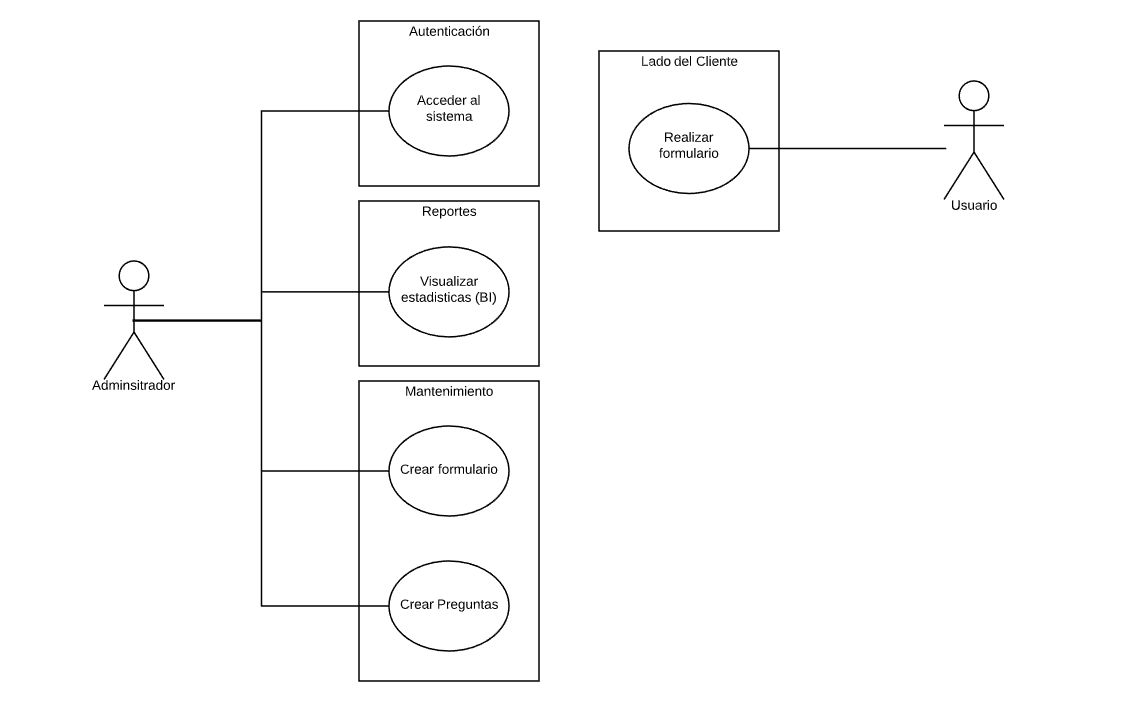
\includegraphics[width=7.5cm]{./Imagenes/use_case} 
		\caption{Use case}
	\end{center}
\end{figure}

\subsection{Diagrama de Arquitectura de la aplicación}
Diagrama de Arquitectura de la aplicación
\begin{figure}[h!]
	\begin{center}
		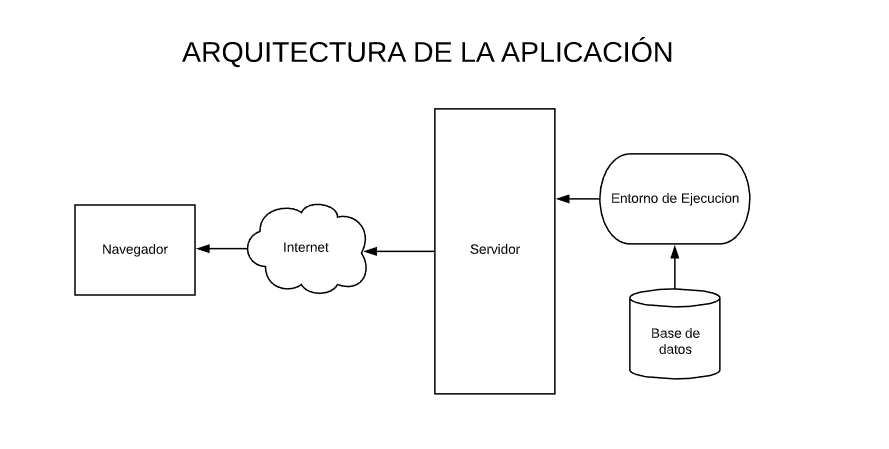
\includegraphics[width=7.5cm]{./Imagenes/bd_architecture} 
		\caption{bd architecture}
	\end{center}
\end{figure}

\subsection{Diagrama de Clases de la aplicación}
Diagrama de Clases de la aplicación
\begin{figure}[h!]
	\begin{center}
		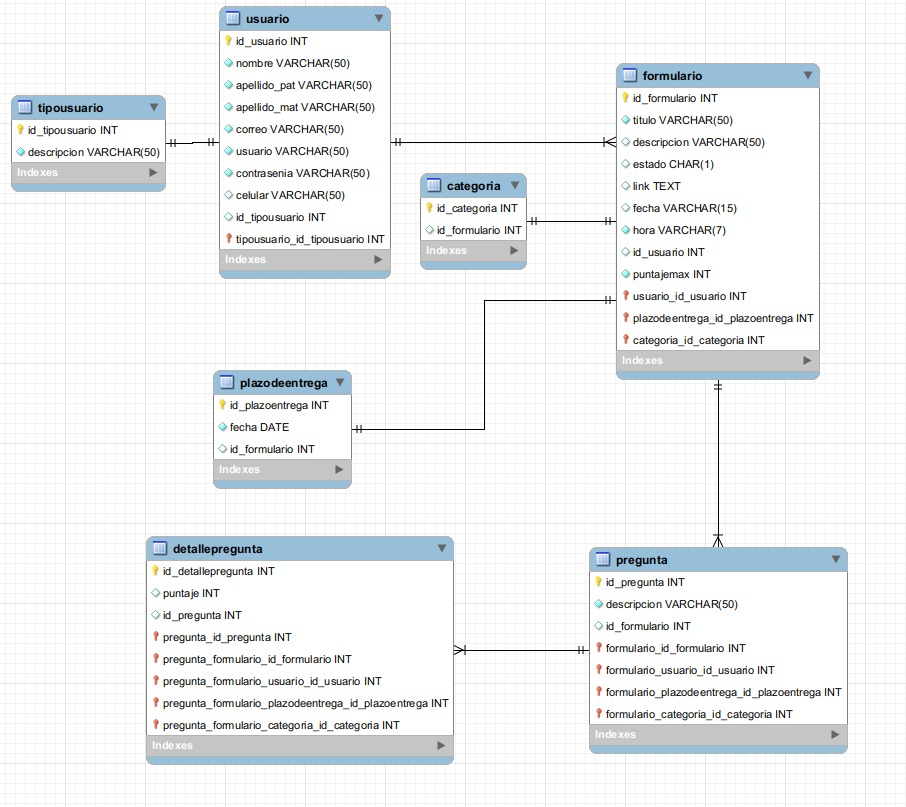
\includegraphics[width=7.5cm]{./Imagenes/diagramclass} 
		\caption{Diagram Class}
	\end{center}
\end{figure}



\end{document}
